\documentclass[border=0pt]{standalone}
\usepackage{tikz}
\usepackage{amsmath,amssymb}
\usetikzlibrary{arrows.meta}
\begin{document}
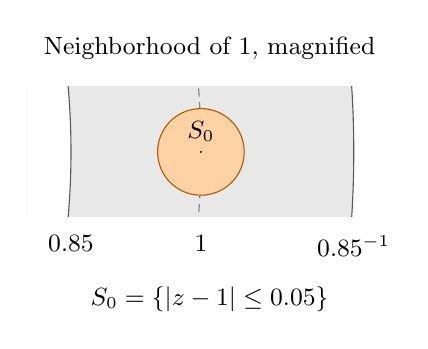
\begin{tikzpicture}[x=11cm,y=11cm,font=\small]
 \begin{scope}
  \clip (0.80,-0.075) rectangle (1.22,0.075);
  \fill[gray!18] (0,0) circle[radius=1.1764706];
  \fill[white] (0,0) circle[radius=0.85];
  \draw[black!65] (0,0) circle[radius=0.85];
  \draw[black!65] (0,0) circle[radius=1.1764706];
  \draw[densely dashed,black!50] (0,0) circle[radius=1];
  \filldraw[fill=orange!35,draw=orange!70!black] (1,0) circle[radius=0.05];
  \fill (1,0) circle[radius=0.0012];
 \end{scope}
 \node at (1.01,0.12) {Neighborhood of $1$, magnified};
 \node[below] at (0.85,-0.085) {$0.85$};
 \node[below] at (1,-0.085) {$1$};
 \node[below] at (1.17647,-0.085) {$0.85^{-1}$};
 \node at (1.01,-0.17) {$S_0=\{|z-1|\leq0.05\}$};
 \node at (1,0.024) {$S_0$};
\end{tikzpicture}
\end{document}
